% Options for packages loaded elsewhere
\PassOptionsToPackage{unicode}{hyperref}
\PassOptionsToPackage{hyphens}{url}
%
\documentclass[
]{article}
\usepackage{amsmath,amssymb}
\usepackage{iftex}
\ifPDFTeX
  \usepackage[T1]{fontenc}
  \usepackage[utf8]{inputenc}
  \usepackage{textcomp} % provide euro and other symbols
\else % if luatex or xetex
  \usepackage{unicode-math} % this also loads fontspec
  \defaultfontfeatures{Scale=MatchLowercase}
  \defaultfontfeatures[\rmfamily]{Ligatures=TeX,Scale=1}
\fi
\usepackage{lmodern}
\ifPDFTeX\else
  % xetex/luatex font selection
\fi
% Use upquote if available, for straight quotes in verbatim environments
\IfFileExists{upquote.sty}{\usepackage{upquote}}{}
\IfFileExists{microtype.sty}{% use microtype if available
  \usepackage[]{microtype}
  \UseMicrotypeSet[protrusion]{basicmath} % disable protrusion for tt fonts
}{}
\makeatletter
\@ifundefined{KOMAClassName}{% if non-KOMA class
  \IfFileExists{parskip.sty}{%
    \usepackage{parskip}
  }{% else
    \setlength{\parindent}{0pt}
    \setlength{\parskip}{6pt plus 2pt minus 1pt}}
}{% if KOMA class
  \KOMAoptions{parskip=half}}
\makeatother
\usepackage{xcolor}
\usepackage[margin=1in]{geometry}
\usepackage{color}
\usepackage{fancyvrb}
\newcommand{\VerbBar}{|}
\newcommand{\VERB}{\Verb[commandchars=\\\{\}]}
\DefineVerbatimEnvironment{Highlighting}{Verbatim}{commandchars=\\\{\}}
% Add ',fontsize=\small' for more characters per line
\usepackage{framed}
\definecolor{shadecolor}{RGB}{248,248,248}
\newenvironment{Shaded}{\begin{snugshade}}{\end{snugshade}}
\newcommand{\AlertTok}[1]{\textcolor[rgb]{0.94,0.16,0.16}{#1}}
\newcommand{\AnnotationTok}[1]{\textcolor[rgb]{0.56,0.35,0.01}{\textbf{\textit{#1}}}}
\newcommand{\AttributeTok}[1]{\textcolor[rgb]{0.13,0.29,0.53}{#1}}
\newcommand{\BaseNTok}[1]{\textcolor[rgb]{0.00,0.00,0.81}{#1}}
\newcommand{\BuiltInTok}[1]{#1}
\newcommand{\CharTok}[1]{\textcolor[rgb]{0.31,0.60,0.02}{#1}}
\newcommand{\CommentTok}[1]{\textcolor[rgb]{0.56,0.35,0.01}{\textit{#1}}}
\newcommand{\CommentVarTok}[1]{\textcolor[rgb]{0.56,0.35,0.01}{\textbf{\textit{#1}}}}
\newcommand{\ConstantTok}[1]{\textcolor[rgb]{0.56,0.35,0.01}{#1}}
\newcommand{\ControlFlowTok}[1]{\textcolor[rgb]{0.13,0.29,0.53}{\textbf{#1}}}
\newcommand{\DataTypeTok}[1]{\textcolor[rgb]{0.13,0.29,0.53}{#1}}
\newcommand{\DecValTok}[1]{\textcolor[rgb]{0.00,0.00,0.81}{#1}}
\newcommand{\DocumentationTok}[1]{\textcolor[rgb]{0.56,0.35,0.01}{\textbf{\textit{#1}}}}
\newcommand{\ErrorTok}[1]{\textcolor[rgb]{0.64,0.00,0.00}{\textbf{#1}}}
\newcommand{\ExtensionTok}[1]{#1}
\newcommand{\FloatTok}[1]{\textcolor[rgb]{0.00,0.00,0.81}{#1}}
\newcommand{\FunctionTok}[1]{\textcolor[rgb]{0.13,0.29,0.53}{\textbf{#1}}}
\newcommand{\ImportTok}[1]{#1}
\newcommand{\InformationTok}[1]{\textcolor[rgb]{0.56,0.35,0.01}{\textbf{\textit{#1}}}}
\newcommand{\KeywordTok}[1]{\textcolor[rgb]{0.13,0.29,0.53}{\textbf{#1}}}
\newcommand{\NormalTok}[1]{#1}
\newcommand{\OperatorTok}[1]{\textcolor[rgb]{0.81,0.36,0.00}{\textbf{#1}}}
\newcommand{\OtherTok}[1]{\textcolor[rgb]{0.56,0.35,0.01}{#1}}
\newcommand{\PreprocessorTok}[1]{\textcolor[rgb]{0.56,0.35,0.01}{\textit{#1}}}
\newcommand{\RegionMarkerTok}[1]{#1}
\newcommand{\SpecialCharTok}[1]{\textcolor[rgb]{0.81,0.36,0.00}{\textbf{#1}}}
\newcommand{\SpecialStringTok}[1]{\textcolor[rgb]{0.31,0.60,0.02}{#1}}
\newcommand{\StringTok}[1]{\textcolor[rgb]{0.31,0.60,0.02}{#1}}
\newcommand{\VariableTok}[1]{\textcolor[rgb]{0.00,0.00,0.00}{#1}}
\newcommand{\VerbatimStringTok}[1]{\textcolor[rgb]{0.31,0.60,0.02}{#1}}
\newcommand{\WarningTok}[1]{\textcolor[rgb]{0.56,0.35,0.01}{\textbf{\textit{#1}}}}
\usepackage{graphicx}
\makeatletter
\def\maxwidth{\ifdim\Gin@nat@width>\linewidth\linewidth\else\Gin@nat@width\fi}
\def\maxheight{\ifdim\Gin@nat@height>\textheight\textheight\else\Gin@nat@height\fi}
\makeatother
% Scale images if necessary, so that they will not overflow the page
% margins by default, and it is still possible to overwrite the defaults
% using explicit options in \includegraphics[width, height, ...]{}
\setkeys{Gin}{width=\maxwidth,height=\maxheight,keepaspectratio}
% Set default figure placement to htbp
\makeatletter
\def\fps@figure{htbp}
\makeatother
\setlength{\emergencystretch}{3em} % prevent overfull lines
\providecommand{\tightlist}{%
  \setlength{\itemsep}{0pt}\setlength{\parskip}{0pt}}
\setcounter{secnumdepth}{-\maxdimen} % remove section numbering
\ifLuaTeX
  \usepackage{selnolig}  % disable illegal ligatures
\fi
\usepackage{bookmark}
\IfFileExists{xurl.sty}{\usepackage{xurl}}{} % add URL line breaks if available
\urlstyle{same}
\hypersetup{
  pdftitle={Guide to statistical methods in R},
  pdfauthor={Pauline Busch},
  hidelinks,
  pdfcreator={LaTeX via pandoc}}

\title{Guide to statistical methods in R}
\author{Pauline Busch}
\date{2024-08-16}

\begin{document}
\maketitle

{
\setcounter{tocdepth}{2}
\tableofcontents
}
Note: For demonstration purposes I am using the a package with 19
medical datasets for teaching reproducible medical research with R. The
package is called ``medicaldata'' and needs to be installed if you would
like to reproduce the results shown in this document in your R-script.

\subsection{Install ggstatsplot}\label{install-ggstatsplot}

If not done already install the package called ggstatsplot. For this
copy the code down below into the console and press enter. You might
need to install other packages as well. Do this in the same fashion
using the install.packages() function.

\begin{verbatim}
## install.packages("ggstatsplot")
\end{verbatim}

\subsection{Load the required R
libraries}\label{load-the-required-r-libraries}

There are many nice libraries that support statistics in R. I recommend
the following:

\begin{Shaded}
\begin{Highlighting}[]
\FunctionTok{library}\NormalTok{(ggstatsplot)}
\end{Highlighting}
\end{Shaded}

In addition to that, we want to load, manipulate and visualize our data
from excel:

\begin{Shaded}
\begin{Highlighting}[]
\FunctionTok{library}\NormalTok{(readxl)}
\FunctionTok{library}\NormalTok{(openxlsx)}
\FunctionTok{library}\NormalTok{(dplyr)}
\FunctionTok{library}\NormalTok{(car)}
\FunctionTok{library}\NormalTok{(ggplot2)}
\FunctionTok{library}\NormalTok{(ggthemes)}
\FunctionTok{library}\NormalTok{(ggpubr)}
\FunctionTok{library}\NormalTok{(ggsci)}
\FunctionTok{library}\NormalTok{(patchwork)  }
\end{Highlighting}
\end{Shaded}

\subsection{Choosing the right statistical
method}\label{choosing-the-right-statistical-method}

\subsubsection{Data preparation}\label{data-preparation}

The first step is to identify whether your data is categorical or
continuous. This will influence your choice of statistical methods.

\begin{itemize}
\tightlist
\item
  Categorical data: Data that represent categories (e.g., gender,
  color).
\item
  Continuous data: Data that represent measurements on a continuous
  scale (e.g., height, weight).
\end{itemize}

Furthermore, you should check for outliers and missing data and decide
how you want to handle these.

\subsubsection{Testing assumptions}\label{testing-assumptions}

Two common assumptions are normality and homogeneity of variances. The
following section demonstrates how to do this in R.

\paragraph{Normality}\label{normality}

Parametric statistical tests assume that the data are normally
distributed.Use the following tests to assess normality:

\begin{itemize}
\item
  \textbf{Shapiro-Wilk Test:} A formal test for normality.\\
  Let's test whether our data is normally distributed. The following
  code shows an example on how to conduct a Shapiro-Wilk Test on the
  previously loaded ``medicaldata''. For comprehension: We want to
  understand whether RBC storage duration and biochemical prostate
  cancer recurrence after radical prostatectomy are associated. RBC age
  is categorized in three groups (1-3) from ``younger'' to ``older''
  depending on storage time (see: RBC.Age.Group). Cancer recurrence can
  be found in the last column (TimeToRecurrence).

  \begin{itemize}
  \tightlist
  \item
    Normality is assumed when p \textgreater{} 0.05.
  \item
    Note: If the Shapiro-Wilk test is performed on individual groups
    separately, it's possible that some groups show normality (p
    \textgreater{} 0.05), while others do not (p \textless{} 0.05). This
    suggests that the assumption of normality for ANOVA may be violated.
  \end{itemize}
\end{itemize}

\begin{Shaded}
\begin{Highlighting}[]
\NormalTok{grouped\_data }\OtherTok{\textless{}{-}} \FunctionTok{split}\NormalTok{(blood}\SpecialCharTok{$}\NormalTok{TimeToRecurrence, blood}\SpecialCharTok{$}\NormalTok{RBC.Age.Group) }\CommentTok{\#data preparation}
\NormalTok{shapiro\_results }\OtherTok{\textless{}{-}} \FunctionTok{lapply}\NormalTok{(grouped\_data, shapiro.test) }\CommentTok{\#lapply() applies the shapiro{-}function to all groups}

\CommentTok{\# without lappy() its more complicated: shapiro\_results \textless{}{-} shapiro.test(grouped\_data[["1"]])}
\end{Highlighting}
\end{Shaded}

\begin{itemize}
\tightlist
\item
  \textbf{Q-Q Plot and Histogram:} A visual methods to check if your
  data follows a normal distribution. The following code shows how you
  can visually check the distribution of your data. This is not
  necessary but might help to comprehend the results of the Shapiro-Wilk
  test and get a feeling for your data.
\end{itemize}

\begin{Shaded}
\begin{Highlighting}[]
\CommentTok{\# How to make a Q{-}Q Plot}
\NormalTok{QQ\_plot }\OtherTok{\textless{}{-}} \FunctionTok{ggplot}\NormalTok{(}\AttributeTok{data =}\NormalTok{ blood, }
                  \FunctionTok{aes}\NormalTok{(}\AttributeTok{sample =}\NormalTok{ TimeToRecurrence, }
                      \AttributeTok{color =} \FunctionTok{factor}\NormalTok{(RBC.Age.Group))) }\SpecialCharTok{+} 
  \FunctionTok{stat\_qq}\NormalTok{() }\SpecialCharTok{+}
  \FunctionTok{stat\_qq\_line}\NormalTok{() }\SpecialCharTok{+}
  \FunctionTok{facet\_grid}\NormalTok{(}\FunctionTok{vars}\NormalTok{(RBC.Age.Group)) }\SpecialCharTok{+}
  \FunctionTok{scale\_color\_futurama}\NormalTok{(}\AttributeTok{name =} \StringTok{"RBC age group"}\NormalTok{)}

\CommentTok{\# How to make a Histogram}
\NormalTok{Histogram }\OtherTok{\textless{}{-}} \FunctionTok{ggplot}\NormalTok{(}\AttributeTok{data =}\NormalTok{ blood, }
                    \FunctionTok{aes}\NormalTok{(}\AttributeTok{x =}\NormalTok{ TimeToRecurrence, }
                        \AttributeTok{fill =} \FunctionTok{factor}\NormalTok{(RBC.Age.Group), }
                        \AttributeTok{color =} \FunctionTok{factor}\NormalTok{(RBC.Age.Group))) }\SpecialCharTok{+}
  
  \FunctionTok{geom\_histogram}\NormalTok{(}\AttributeTok{bins =} \DecValTok{15}\NormalTok{) }\SpecialCharTok{+}
  \FunctionTok{facet\_grid}\NormalTok{(}\FunctionTok{vars}\NormalTok{(RBC.Age.Group)) }\SpecialCharTok{+}
  \FunctionTok{scale\_fill\_futurama}\NormalTok{(}\AttributeTok{alpha =} \FloatTok{0.65}\NormalTok{, }\AttributeTok{name =} \StringTok{"RBC age group"}\NormalTok{) }\SpecialCharTok{+}
  \FunctionTok{scale\_color\_futurama}\NormalTok{(}\AttributeTok{name =} \StringTok{"RBC age group"}\NormalTok{) }
  
\CommentTok{\# Combine Q{-}Q Plot and Histogram}
\NormalTok{combined\_plot }\OtherTok{\textless{}{-}}\NormalTok{ QQ\_plot }\SpecialCharTok{+}\NormalTok{ Histogram }\SpecialCharTok{+} 
  \FunctionTok{plot\_layout}\NormalTok{(}\AttributeTok{ncol =} \DecValTok{2}\NormalTok{) }\SpecialCharTok{\&} \FunctionTok{theme}\NormalTok{(}\AttributeTok{legend.position =} \StringTok{"bottom"}\NormalTok{)}

\FunctionTok{print}\NormalTok{(combined\_plot)}
\end{Highlighting}
\end{Shaded}

\includegraphics{Guide-to-statistical-methods-in-R_files/figure-latex/unnamed-chunk-6-1.pdf}

\paragraph{Homogeneity of variances}\label{homogeneity-of-variances}

Some tests require that the variances between groups are equal. Use
Levene's Test to check for equality of variances.

\begin{itemize}
\item
  \textbf{Levene's Test:} A tests that compares the variances between
  groups.\\
  The following code demonstrates how to conduct the Levene's test in R.

  \begin{itemize}
  \tightlist
  \item
    Homogeneity of variances is assumed when `Pr(\textgreater F)'
    (p-value) \textgreater{} 0.05.
  \end{itemize}
\end{itemize}

\begin{Shaded}
\begin{Highlighting}[]
\NormalTok{levene\_results }\OtherTok{\textless{}{-}} \FunctionTok{leveneTest}\NormalTok{(TimeToRecurrence }\SpecialCharTok{\textasciitilde{}} \FunctionTok{factor}\NormalTok{(RBC.Age.Group), }\AttributeTok{data =}\NormalTok{ blood)}
\end{Highlighting}
\end{Shaded}

\subsubsection{The approporiate statistical test for your research
question}\label{the-approporiate-statistical-test-for-your-research-question}

Once you've checked the assumptions, the next step is to choose the
appropriate statistical test based on your data type and research
question. The decision tree in the next chapter can help with that. If
you are not sure or need help you can ask ChatGPT to assist you with
this (e.g., first prompt: ``Can you find me a suitable statistical
method to analyse my experiment?'' - then fill out all the information
ChatGPT asks from you).

\subsubsection{Decision tree}\label{decision-tree}

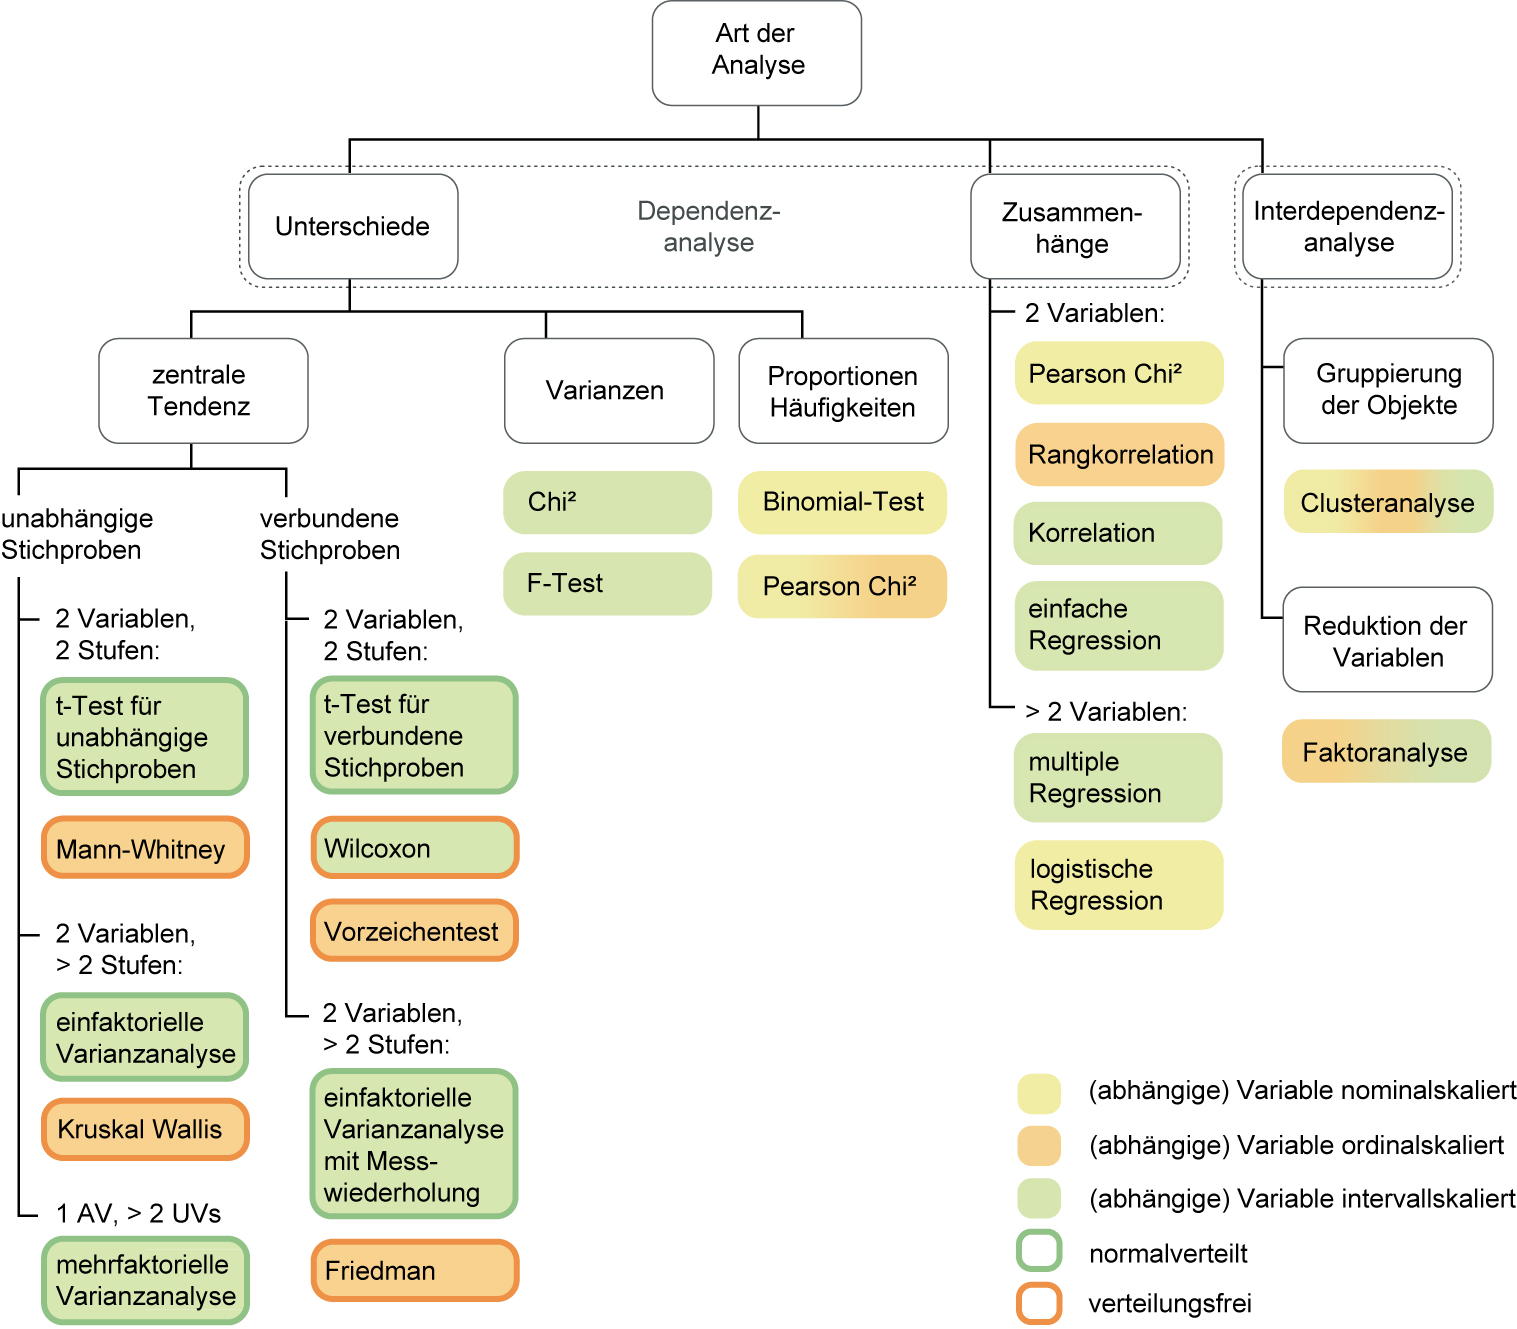
\includegraphics{https://www.methodenberatung.uzh.ch/static/entscheidbaum/entscheidbaum.jpg}

\subsection{Statistical methods}\label{statistical-methods}

\subsubsection{Kruskal-Wallis Test}\label{kruskal-wallis-test}

\subsection{Post-hoc analysis}\label{post-hoc-analysis}

\subsubsection{Dunn's Test}\label{dunns-test}

\end{document}
